\section{PWM Circuit Simulation Results}
\Cref{fig:pwmcircuit} gives the LTspice circuit for the PWM generator and \cref{fig:pwm-output} gives its output and the ramp voltage over the capacitor.

The output voltage is not at the nominal frequency of 100kHz, but rather at \SI{89.6}{\kilo\hertz}. 

$V_C$ is \SI{3.87}{\volt}p--p, close to the design value and within the 4V limit.


\begin{figure}
	\centering
	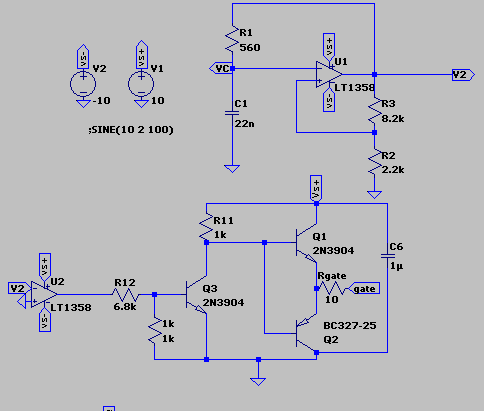
\includegraphics[width=\linewidth]{img/PWMCircuit}
	\caption{PWM Circuit}
	\label{fig:pwmcircuit}
\end{figure}

\begin{figure}
	\centering
	\includegraphics[width=\linewidth]{"img/PWM Output"}
	\caption{Output of PWM circuit}
	\label{fig:pwm-output}
\end{figure}

\subsection{PWM Generator Simulation Results}
% The simulation results presented should validate that the design meets the specification.
% Include diagrams and figures to support your presentation of results.
% In addition to presenting the simulation results include an answer to the following questions. Make sure that the answers to the questions are clearly indicated in your report.
\subsubsection{Explain the design basis for the choice of op-amp power supply voltages, +Vs and -Vs? What is the minimum value which could be used for these?}
The op-amp power supply voltages must be large enough that the saturation voltage of the op-amp is enough to allow for the circuit to operate successfully. Given that we wanted to use the largest possible range of reference voltages, \SI{4}{\volt}p--p, the supply voltages would had have to have been greater than $\pm 2+1=\pm3 V$. They would need to be greater than this however in order to use a resistive divider with reasonable resistances.

We chose 10 V because it was the nominal input voltage to the converter and having one input voltage level for the whole circuit would make supplying power much easier.
\subsubsection{What is the power consumption of the PWM circuit? What is this power used for?}
\begin{table}[h]
	\centering
	\caption{Power Consumption}
	\begin{tabular}{ll}
		\toprule
		Component&Power Consumed \si{\watt}\\
		\cmidrule(r){1-1}\cmidrule(l){2-2}
		PWM Power Supply & $\num{-110.49e-3}+\num{-171.74e-3}=\num{-0.28223}$\\
		Converter Power Supply & \num{-5.1519}\\
		Converter Output Voltage & \num{4.6769}\\
		\bottomrule
	\end{tabular}
	\label{tab:pwm power}
\end{table}
The power consumption of the PWM circuit is as given in \cref{tab:pwm power}. This power is dissipated among the resistors, capacitors and MOSFETS, and is used to power the op amps.
\subsubsection{What is the effect of the PWM circuit power consumption on the converter efficiency?}
%Quantify your answer.
The power consumption of the PWM generator has a small impact on the overall efficiency. The total power supplied to the circuit is \SI{0.28223}{\watt} which will lower the overall converter efficiency: from 90.7\% to 86.0\%.

\subsection{PWM Generator \& Buck Converter Results}
% The simulation results presented should validate that the design meets the specification.
% Include diagrams and figures to support your presentation of results.

\begin{figure}
	\centering
	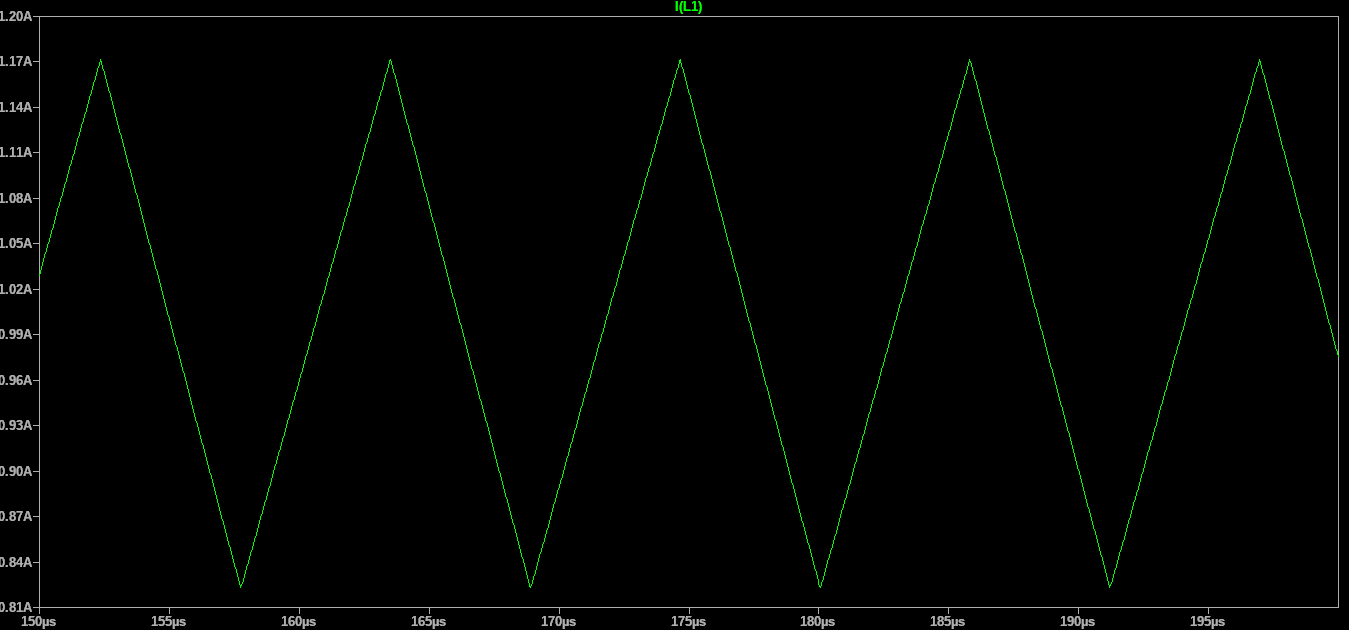
\includegraphics[width=\linewidth]{img/IL}
	\caption{Inductor current}
	\label{fig:il}
\end{figure}

\begin{figure}
	\centering
	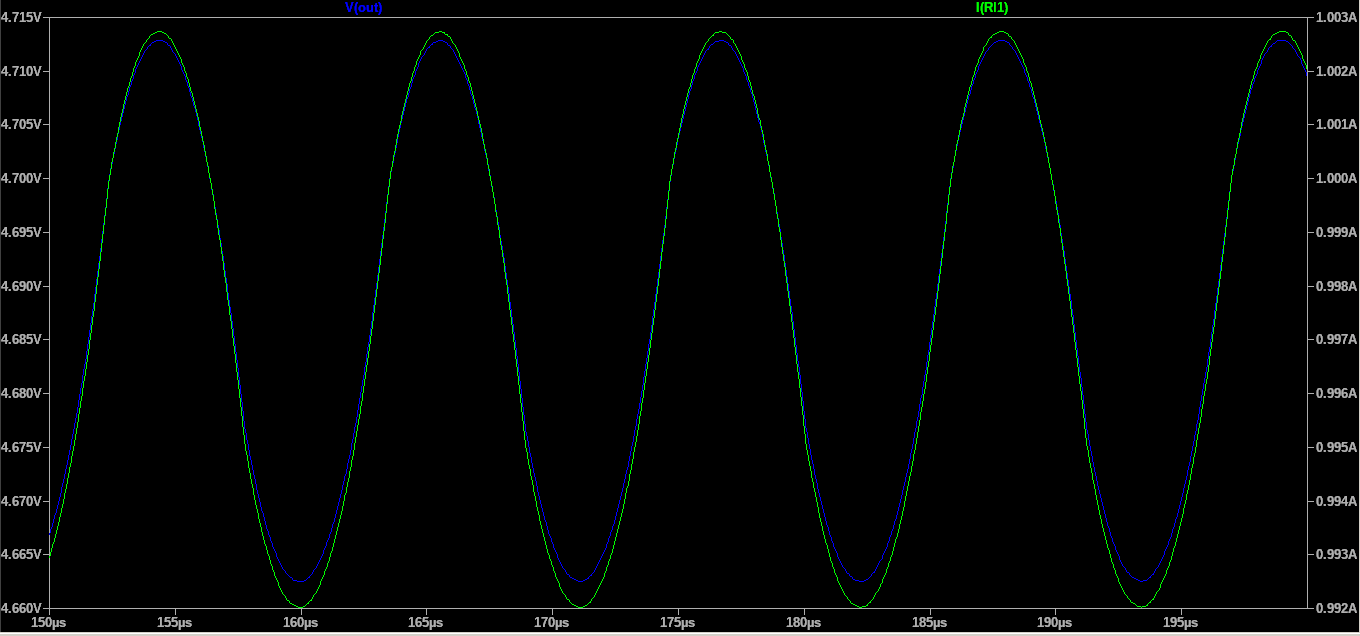
\includegraphics[width=\linewidth]{img/VoIo}
	\caption{Output voltage and current for PWM and converter circuit}
	\label{fig:voio}
\end{figure}

\Cref{fig:il} gives the inductor current and \cref{fig:voio} the output voltage and current for the combined circuit. The input voltage was 10V, the duty cycle was 0.5 and the load was \SI{4.7}{\ohm}.

The output voltage ripple is just over the specified value, \SI{50.2}{\milli\volt} instead of \SI{50}{\milli\volt}. The output current is 997.34 mA, nearly exactly the specified 1 A, and the output voltage is 4.6875 V.


% In addition to presenting the simulation results include an answer to the following questions. Make sure that the answers to the questions are clearly indicated in your report.
\subsubsection{What is the relationship between output voltage and reference voltage?}
% You could investigate this with a graph of output voltage vs. reference voltage.
\begin{figure}
	\centering
	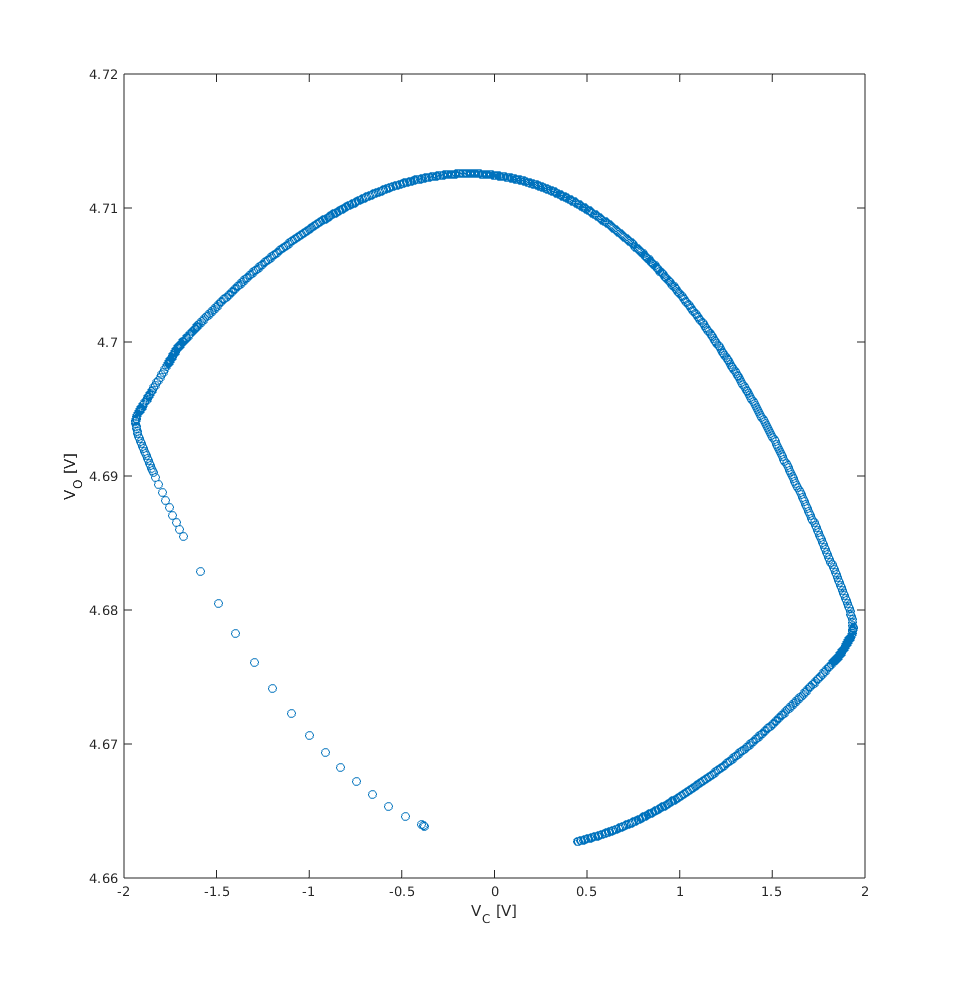
\includegraphics[width=\linewidth]{VoVc.png}
	\caption{Graph of output voltage vs reference voltage for one switching cycle.}
	\label{fig:vovc}
\end{figure}
The output voltage and reference voltage appear to be related in a manner where the output voltage depends not only on the reference voltage but also on what direction the output voltage is travelling, similar to the current-voltage graph for a transformer.
\subsubsection{Could the same PWM circuit be used to drive the converter at 10 times your design frequency? What might limit the maximum frequency of operation of this circuit?}

The fall time of the circuit is $\approx\SI{100}{\nano\second}$ and the rise time is $\approx\SI{90}{\nano\second}$. At a frequency of $f_s\times 10=\SI{1}{\mega\hertz}$, the rise and fall times of the circuit are about 10\% the period of the converter. This would allow for only a reduced set of duty cycles if the RC product can be changed.

The maximum frequency of operation of this circuit could be limited by the slew rate of the op amps and the frequency at which the capacitors become inductive.